\documentclass[french,a4paper,titlepage]{article}
\usepackage{xunicode}
\usepackage{fontspec}
\usepackage[frenchb]{babel}
\usepackage{graphicx}
\usepackage{listings}
\usepackage[T1]{fontenc}
\usepackage{kpfonts}


\renewcommand*{\familydefault}{\sfdefault}

\renewcommand{\nobreakspace}{\nobreak\ }

\title{Projet HADL: Conception et réalisation}
\author{Julien Durillon \and Alexandre Garnier}
\date{\today}


\lstset{
   language=XML,
   basicstyle=\scriptsize,
   numbers=left,
   numberstyle=\scriptsize,
   stepnumber=1,
   showspaces=false,
   showstringspaces=false,
   morekeywords={configuration,composant,service,port,entrypoint,connector},
   tabsize=2
}


\begin{document}

	\maketitle

	\tableofcontents\clearpage
	
	\section*{Introduction}
	\addcontentsline{toc}{section}{Introduction}

	  Dans le cadre du module de Composants, nous avons eu à développer une
	  solution logicielle permettant une représentation et une gestion efficaces
	  d'une architecture à composants; ce depuis l'exécution d'une application
	  basée sur l'architecture proposée jusqu'à la méta-méta-modélisation de la
	  solution apportée, c'est à dire la modélisation du paradigme
	  \emph{composant}.

    Dans ce cadre, nous nous sommes intéressés à l'implémentation à base de
    composants d'une architecture Client-Serveur.
    
    Nous avons dès lors choisi de suivre une approche descendante
    (\emph{top-down}) du travail à effectuer. C'est à dire que nous sommes
    partis des concepts permettant la gestion des composants de manière
    générale, pour ensuite les utiliser afin de parvenir à l'implémentation de
    l'application Client-Serveur à proprement parler.

	\section{Niveau M2}
	
		Pour commencer, nous avons défini notre système en suivant la méthode top-down, pendant la conception comme pendant l'implémentation.
	
		\subsection{Conception}
		\normalfont
			Ce niveau décrit l'architecture d'un système à composants.
		
			%Diagramme général M2
			\begin{figure}[ht]
				\centering
				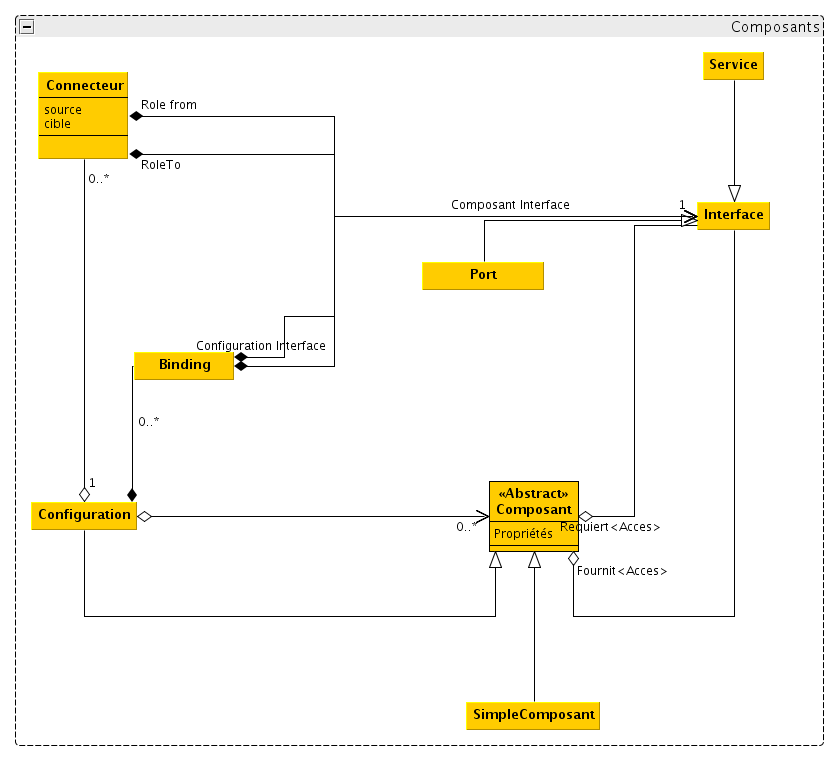
\includegraphics[width=1.00\textwidth]{M2.png}
				\caption{M2: Modèle de l'architecture à composant}
				\label{fig:m2}
			\end{figure}

			La figure \ref{fig:m2} exprime les différents éléments de l'architecture à
			composants et leurs liens.
		
			\paragraph{Composant}
			
				Cette classe est abstraite et doit permettre à n'importe quelle
				classe de se déclarer comme composant en l'étendant.
				
			\paragraph{SimpleComposant et Configuration}
			
				Ces deux classes --- avec Composant--- permettent de fournir un
				pattern composite, demandé par la spécification. Configuration
				est l'objet composite.
			
			\paragraph{Interface}
			
				Un Composant possède des interfaces, qui sont de deux types: Port et
				Service. Ces interfaces sont soit fournies soit requises. Voir page
				\pageref{def:reqfour} pour les interfaces fournies et requises.
				
				
			\paragraph{Connecteur}
			
				Un connecteur connecte une interface fournie (roleFrom) d'un
				composant, et une interface requise (roleTo) d'un autre. Les
				interfaces doivent être de différents composants.
				
				Les connecteurs sont définis dans les configurations. Ils ne
				connectent que les interfaces des composants contenus par la
				configuration.
				
			\paragraph{Binding}
			
				Un Binding fonctionne comme un connecteur, à la différence qu'il
				connecte une interface d'une configuration à une interface d'un de
				ses composants. Les deux interfaces connectées doivent être toutes
				les deux fournies ou requises.
				
				L'appel d'une interface requise d'une configuration doit être passé
				à l'interface requise du composant connecté.

				La mise à disposition d'une interface fournie d'un composant doit
				donner lieu à la mise à disposition de l'interface fournie de sa
				configuration associée.
				
			\paragraph{Requise vs fournie}
				\label{def:reqfour}
				Une interface requise est une interface par laquelle on va pouvoir
				passer des messages à un composant. Son nom vient du fait qu'elle va
				requérir des informations.
				
				Une interface requise est une interface qui va fournir des
				informations.
				
				Quand une interface requise est connectée à une interface fournie,
				le connecteur se déclenchera quand l'interface fournies se déclarera
				prête à envoyer des informations.
				
			
			
		\subsection{Implémentation}
		
		Au niveau de l'implémentation, certaines notions ne se présentent plus de
		la même façon:
		
		\subsubsection{Interfaces}
		
			Les interfaces des composants ne sont pas des objets à part, mais sont
			les méthodes et les attributs (resp. service et port) de l'objet
			représentant un composant.
			
		\subsubsection{Composant et Configuration}
		
			Nous avons implémenté les composants comme explicité sur le diagramme.
			Ainsi, nous avons implémenté un pattern composite.
			
			Notre but était de mettre un maximum du code traitant des envois de
			message dans l'implémentation du M2. Ainsi, le M1 ne contiendra que le
			code spécifique.
			
			Pour les messages, nous avons utilisé le pattern Observer-Observable
			comme fournit par java. Les figures \ref{fig:obsimpl} et
			\ref{fig:obsimpl2} décrivent l'architecture
			d'une configuration ainsi que son fonctionnement.
			
			\begin{figure}[ht]
				\centering
				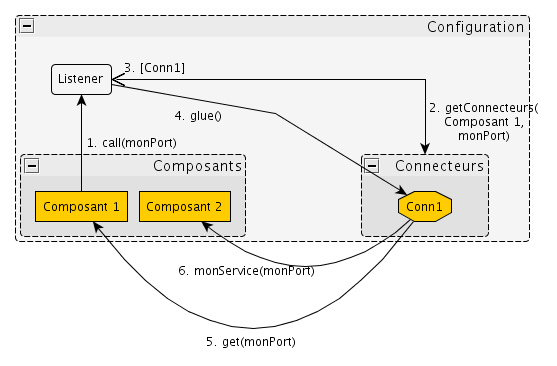
\includegraphics[width=1.00\textwidth]{obsimpl.png}
				\caption{Architecture et fonctionnement d'une configuration: les
				          connecteurs}
				\label{fig:obsimpl}
			\end{figure}
			
			\begin{figure}[ht]
				\centering
				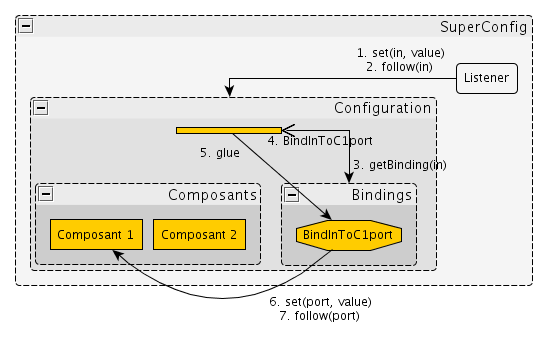
\includegraphics[width=1.00\textwidth]{obsimpl2.png}
				\caption{Architecture et fonctionnement d'une configuration: les
          			  bindings}
				\label{fig:obsimpl2}
			\end{figure}
			
			
	\section{Conception et implémentation du M1 : système client-serveur}
	
	  L'implémentation des concepts liés à la gestion des composants ayant été
	  assurée au niveau M2, l'implémentation propre du système Client-Serveur est
	  dès lors rendue bien plus aisée.
	  
    Ainsi, et dans l'optique de séparer composants et architecture du système,
    nous avons choisi de disposer d'un pool de composants et de connecteurs
    d'une part, et d'un fichier \emph{architecture.xml} décrivant les liens au
    sein de cette architecture d'autre part.
    
    \subsection{Gestion et définition des composants et connecteurs}
    
      
    
    \subsection{Fichier \emph{architecture.xml}}
    
      
	
		Grâce aux élément définis dans la section précédente, nous n'avons plus grand chose à implémenter.
		
		Le contenu du système Client Serveur est donc un jar se composant de :
		
		\begin{verbatim}
|-- fr
|   `-- alma
|       `-- hadlm1cs
|           |-- components
|           |   |-- Client.class
|           |   |-- ConnManager.class
|           |   `-- Database.class
|           |-- configurations
|           |   |-- CSSystem.class
|           |   `-- Server.class
|           `-- connectors
|               |-- ConnPSIdent.class
|               `-- ConnSSIdent.class
`-- META-INF
    `-- architecture.xml
		\end{verbatim}
		
		
		Le fichier architecture.xml (exposé dans la figure \ref{fig:architecture.xml}) décrit l'architecture du système. Les classes contenues dans le jar implémentent chaque élément, et sont annotées de façon à pouvoir faire le lien entre un composant du fichier xml et une classe fournie.
		
		Ce fonctionnement permet une très bonne réutilisabilité du code.
		
		
		\begin{figure}[htb]
			\centering
			\lstinputlisting{architecture.xml}
			\caption{Contenu du fichier architecture.xml}
			\label{fig:architecture.xml}

		\end{figure}
	
	\section{Le framework, ou comment tout faire fonctionner}
	
		Pour faciliter la réutilisation et le développement des systèmes au niveau M1, nous avons développé un framework. La figure \ref{fig:framework} montre l'agencement des différents éléments --- M1, M2, framework\dots --- qui constituent une application à composants.
		
		Pour lancer un système, il suffit de lancer le framework en lui passant en paramètre le chemin vers le jar du système. Le framework va se charger de lire le fichier architecture.xml, puis charger les classes requises, et lancer le système.
		
		Nous avons introduit l'élément \emph{entrypoint} dans le document, qui définit le nom du service à appeler en premier, et qui référence la méthode qui sera appelée en premier lors du lancement du système après sa construction.
		
		\begin{figure}[htb]
			\centering
			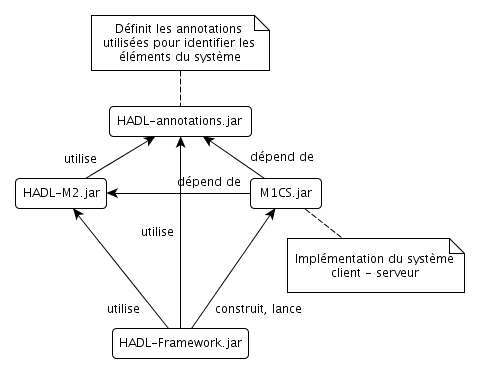
\includegraphics[width=0.8\textwidth]{./framework.png}
			\caption{Dépendances entre les éléments du framework}
			\label{fig:framework}
		\end{figure}
	
	
	\section{Refaisons tout depuis tout en haut}
	
		Après nous être intéressés à la modélisation générique d'un système à composant, à la modélisation de son implémentation et à son implémentation effective, nous avons repris la modélisation depuis le M3 (au niveau du méta-méta-modèle). Nous avons suivi la méthode top-down encore une fois pour générer le M2 puis le M1, en version plus complète.
		
		La figure \ref{fig:M3} illustre notre définition du niveau M3.
		
		\begin{figure}[htb]
			\centering
			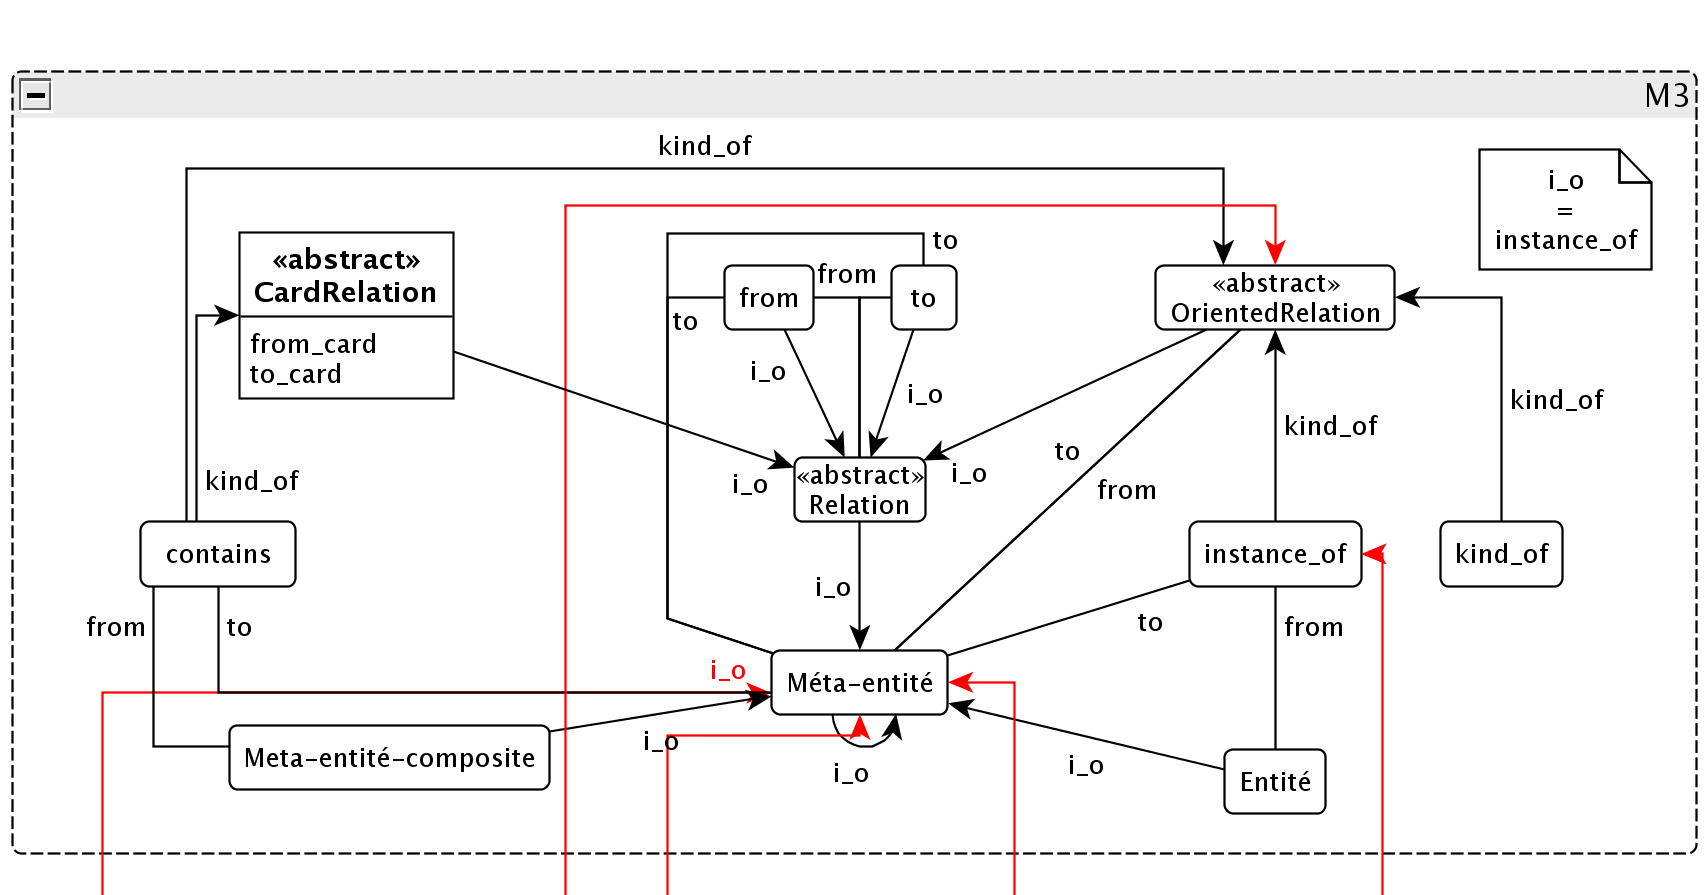
\includegraphics[width=\textwidth]{m3.png}
			\caption{Modélisation du niveau M3}
			\label{fig:M3}
		\end{figure}
		
		\subsection{Description du niveau M3}
		
		
			Le niveau M3 doit permettre de définir les niveaux M2 et M1, et de se définir lui même. Tout commence donc avec la création de l'élément \emph{Méta-entité}. Cet élément est l'ancêtre de tous les autres.
			
			\subsubsection{instance\_of}
			
				L'élément suivant à définir est la relation \emph{instance\_of} qui définit une relation d'instanciation entre une entité et une méta-entité. Une entité A définie comme une instance of une entité B aura tous les attributs de l'entité B. L'élément \emph{Méta\_entité} est une instance de lui même.
				
				La relation \emph{instance\_of} n'est pas cumulative: un élément ne peut pas être instance de plusieurs autres éléments; elle est néanmoins transitive: si \verb!A instance_of B! et \verb!B instance_of C!, alors \verb!A instance_of C!; pour finir, elle n'est pas symétrique: si \verb!A instanceof B! alors \verb!B instance_of A! n'est pas possible.
				
			\subsubsection{Relation, OrientedRelation et CardRelation}
			
				Nous pouvons maintenant définir les relations orientées et avec cardinalité comme des instances de \emph{Méta\_entité}.
				Ces relations sont représentées par la suite par des flèches portant le nom de la relation utilisée.
				
				Les relations \emph{from} et \emph{to} utilisées uniquement au niveau M3 permettent de définir l'orientation d'une relation. le côté flèche sera celui de la relation \emph{to} tandis que l'autre sera celui de la relation \emph{from}. Ces relations sont définies entre une Relation et une Méta\_entité.
				
				Une relation orienté ou avec cardinalité n'est pas symétrique. Une relation avec cardinalité permet de définir combien de fois une entité (ou ses instances) peut être impliquée dans la relation.
				
			\subsubsection{kind\_of}
			
				La relation orientée \emph{kind\_of} permet de définir une méta entité comme étant un équivalent d'une autre méta entité; cette relation est transitive, et permet de restreindre ou d'ajouter des attributs à une entité.
				
				\paragraph{instance\_of} Nous pouvons donc définir cette relation comme un type
		
		
	
	
	
	
\end{document}
